% DESENVOLVIMENTO DA APLICAÇÃO-------------------------------------------------------------------

\chapter{DESENVOLVIMENTO DA APLICAÇÃO}
A proposta para este trabalho foi a construção de uma aplicação que ficaria responsável
por aguardar e coletar as coordenadas geográficas dos pedidos gerados no estabelecimento,
juntamente com o desenvolvimento de um servidor encarregado de gerenciar os pedidos como entregas
com um painel de controle para geração de lotes de entregas e o desenvolvimento de um módulo destinado ao motoboy, no qual consegue observar, em um mapa, a posição e pontos de parada que devem ser percorridos no lote disponível para entrega, tudo isso em tempo real.

%%% Rev-Madalozzo: Aqui no módulo de gerenciamento sugiro você listar todos os pacotes de terceiros que é util e que você utilizou na tua aplicação. Por exemplo, na aula usamos o AdminLTE, caso tu uso algum módulo de terceiros lista neste Capítulo
\section{Módulo de gerenciamento}
Ao utilizar o comando \textit{composer create-project --prefer-dist laravel/laravel delivery-routes} no Cmder, dentro de uma pasta no sistema operacional destinada a programação da aplicação, foi criada a estrutura base do projeto, cedida pelo Laravel, apresentada na \autoref{fig:base-projeto}. A facilidade na criação do projeto se deve ao Cmder, que torna o trabalho no sistema operacional da Microsoft mais agradável, com essa ferramenta é possível rodar comandos do Linux e MAC que são baseados em UNIX para o Windows. Embora nas versões mais recentes do Windows (>= 8.1) já tenha o Power Shell que atende bem a maiorias de comandos UNIX (que são essenciais para desenvolvedores) ainda sim é totalmente recomendado utilizar alguma ferramenta que nivela estes pontos.

\begin{figure}[H]
    \centering
    \caption{Estrutura Laravel}
    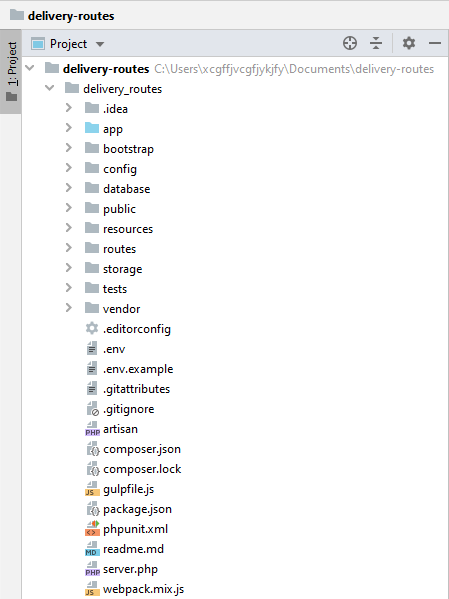
\includegraphics[width=0.6\textwidth]{./dados/figuras/fig6}
    \fonte{Autor}
    \label{fig:base-projeto}
\end{figure}

\begin{figure}[H]
    \centering
    \caption{Delivery Routes - Página inicial}
    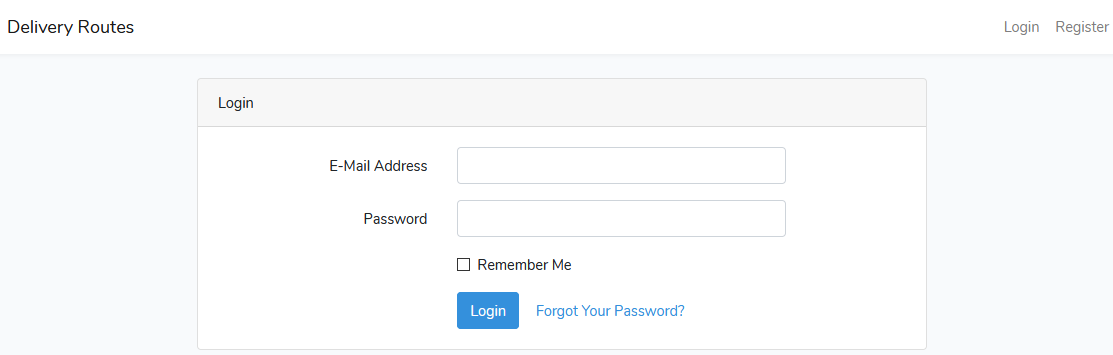
\includegraphics[width=0.9\textwidth]{./dados/figuras/fig7}
    \fonte{Autor}
    \label{fig:apphome}
\end{figure}

\subsection{Coleta de dados}

\subsection{Painel de gerenciamento}

\subsection{Consulta de dados}

\section{Módulo de entrega}